\begin{titlepage}

\centering \parindent=0pt
\newcommand{\HRule}{\rule{\textwidth}{1mm}}
\vspace*{\stretch{1}} \HRule\\[0.7cm]\Huge\bfseries
30010 - Programmeringsprojekt \\[0.7cm] % Kursusnummer og navn
Reflexball\\ % Titel
\HRule\\[2cm]  
\Large
Gruppe 3
\\
\large
Martin Boye Brunsgaard, s144012(1)	\\
Tore Gederaas Kanstad, s144021(2) \\
Peter Asbjørn Leer Bysted, s144045(3) \\
\begin{figure}[h]
\begin{center}
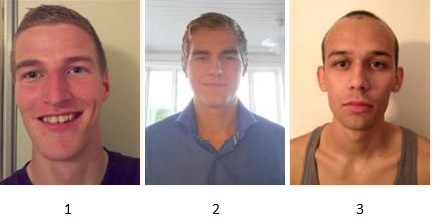
\includegraphics[scale=0.6]{img/faces.jpg}
\end{center}
\end{figure}

\vspace*{\stretch{1}} \normalsize

Alle medlemmer har været tilstede under øvelserne, og deltaget i udarbejdelse af journalerne. Ydermere har arbejdet været fordelt ligeligt over gruppemedlemerne, og løst i fællesskab. Rapporten er blevet udarbejdet og gennemlæst i kollektiv.
\vspace*{\stretch{1}}
\begin{flushleft}
Tecnical University of Denmark DTU\\ % Uddannelsesinstitusion
National Space Institute\\ 
30010 - Programming Project\\ % Kursusnummer og navn
25.06.2015 %Måned og år
\end{flushleft}
\end{titlepage}
\newpage
\renewcommand{\abstractname}{Abstract}
\begin{abstract}

This report covers the reflexbal game, which is a mandatory part of the B.Sc. EE course 30010 Programming Project.\\ The report documents the entirety of this course, the journals and the final product, Reflexball. The first few days The 3 assignements were combined into one circuit and implemented on a Basys2 Spartan FPGA board.
\end{abstract}
\newpage
\tableofcontents


\newpage